\begin{exercice*}
    On considère le programme de calcul suivant.
    \myProgCalcul{$\leadsto$}{Programme}{%
        \ProgCalcul[Enonce,ThemePerso]{%
            Choisir un nombre,%
            Augmenter le nombre de 5,%
            Multiplier le résultat par 4,%
            Ôter le quadruple du nombre de départ,%
            Ôter 10 et annoncer le résultat,%
        }
    }
    \begin{enumerate}
        \item Applique ce programme de calcul à 5 et 2,3.
        \item Que remarques-tu ?
        \item Pour chaque étape du programme, complète le diagramme par des expressions simplifiées.

              \medskip
              \tikzstyle{fond}=[rectangle,draw,rounded corners=4pt,very thick]
              \tikzstyle{quadri}=[rectangle, draw, rounded corners=4pt, fill=gray!30, text=black, minimum width=15mm, minimum height=7mm]
              \tikzstyle{cercle}=[circle,draw,rounded corners=4pt,fill=gray!30,text=black,radius=7mm]
              \tikzstyle{dep}=[-,dotted,very thick,>=latex]
              \tikzstyle{vers}=[->,dotted,very thick,>=latex]
              \hspace*{-10mm}
              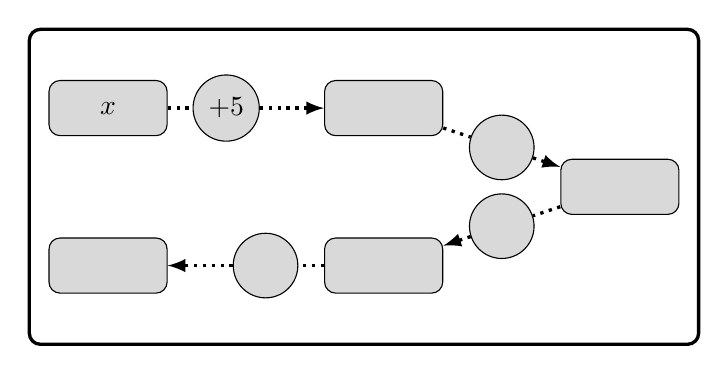
\begin{tikzpicture}[scale=1]
                  \draw[fond] (-11,1) rectangle (-2.5,-3);
                  \node[quadri] (A) at (-10,0) {$x$};
                  \node[cercle] (B) at (-8.5,0) {$+5$};
                  \node[quadri] (C) at (-6.5,0) {\phantom{$r$}};
                  \node[cercle] (D) at (-5,-0.5) {\phantom{$+r$}};
                  \node[quadri] (E) at (-3.5,-1) {\phantom{$r$}};
                  \node[cercle] (F) at (-5,-1.5) {\phantom{$+r$}};
                  \node[quadri] (G) at (-6.5,-2) {\phantom{$r$}};
                  \node[cercle] (H) at (-8,-2) {\phantom{$+r$}};
                  \node[quadri] (I) at (-10,-2) {\phantom{$r$}};
                  \draw[dep] (A)--(B);
                  \draw[vers] (B)--(C);
                  \draw[dep] (C)--(D);
                  \draw[vers] (D)--(E);
                  \draw[dep] (E)--(F);
                  \draw[vers] (F)--(G);
                  \draw[dep] (G)--(H);
                  \draw[vers] (H)--(I);
              \end{tikzpicture}

              \medskip
        \item Conclus.
    \end{enumerate}
\end{exercice*}
\begin{corrige}
    %\setcounter{partie}{0} % Pour s'assurer que le compteur de \partie est à zéro dans les corrigés
    %\phantom{rrr}    
    \dots
\end{corrige}

